\documentclass[a4paper,11pt]{article}
\usepackage[utf8]{inputenc}

\usepackage{comment}

\usepackage[
backend=biber,
style=alphabetic,
sorting=ynt
]{biblatex}
\addbibresource{references.bib}
\nocite{grimett}
\nocite{ihesduminil}
\nocite{bollobas}
\nocite{tassion}

\usepackage{enumerate}
\usepackage{mathrsfs}
\usepackage{amsthm}
\usepackage{amsfonts}
\usepackage{amsmath}
\usepackage{amssymb}
\usepackage{graphicx}
\usepackage{tikz}
% adjust the margins
\usepackage[margin=1.0in]{geometry}
\usepackage{hyperref}

\usepackage{listings}

\lstset{
  aboveskip=1ex,
  backgroundcolor=\color{gray!25},
  basicstyle=\ttfamily\small,
  belowskip=1ex,
  breaklines=true,
  columns=fullflexible,
  framerule=0pt,
  framexrightmargin=0em,
  framexleftmargin=0em,
  numbers=left,
  numberstyle=\footnotesize\sffamily,
  tabsize=2
}

\theoremstyle{plain}
\newtheorem{theorem}{Theorem}[section]
\newtheorem*{theorem*}{Theorem}
\newtheorem{lemma}[theorem]{Lemma}
\newtheorem*{lemma*}{Lemma}
\newtheorem{corollary}[theorem]{Corollary}
\newtheorem*{corollary*}{Corollary}
\newtheorem{proposition}[theorem]{Proposition}
\newtheorem*{proposition*}{Proposition}

\theoremstyle{definition}
\newtheorem{definition}[theorem]{Definition}
\newtheorem{definition*}[theorem]{Definition}
\newtheorem{assumption}[theorem]{Assumption}

\theoremstyle{remark}
\newtheorem*{remark}{Remark}

\def\msquare{\mathop{\scalerel{\Box}{}}}

\graphicspath{ {./images/} }

\title{Bernoulli bond percolation on the $\mathbb{Z}^d$ lattice}
\author{Antoine Colonna d'Istria}
\date{28 May 2021}

\begin{document}

\maketitle
\begin{abstract}
    In this memoir, we will study open clusters of the bond percolation on a n-dimensional cubic lattice. At some point, there is a transition phase phenomena where above some value, there is an infinite cluster almost surely, and below there is never an infinite cluster. The diameters of the open clusters decays exponentially for p below this critical value. We show that the critical probability for dimension 2 is equal to one half and that no infinite cluster exists at this value. A simulation program was created for the purpose of this memoir using methods such as the breadth-first search algorithm to find open clusters.
\end{abstract}

\tableofcontents
\newpage %change can break

\section{Introduction}
What is percolation? We can describe percolation as the study of the behavior of graphs where we remove a certain number of edges with a given probability $p \in [0,1]$. Such removed edges are called ``open'', and those remaining are called ``closed'' edges.

The study of percolation have different applications, such as to study the traffic of a city, in ecology with the fragmentation of animal habitats, for compartmental models in epidemiology (going further than a simple SIR model), and in physics with ferromagnetism and electrical networks.

More precisely, we will be interested in the study of open clusters of such a graph and how it behaves in relation with the probability $p$ chosen. There will be what we call a critical probability $p_c$ that divides the problem in three cases.

We will be only interested by the bond percolation of the lattice $\mathbb{Z}^d$, but we can see that percolation theory can be applied outside of this particular case, for other types of lattices, such as those we can see in Figure \ref{fig:lattices}.

\begin{figure}
\centering
\caption{Examples of lattices}
\begin{tabular}{cc}
  Honeycomb & $p_c = 1 - 2\sin(\frac{\pi}{18})$ \\
  Triangular & $p_c = 2\sin(\frac{\pi}{18})$ \\
  Truncated square & $4p_c^3+3p_c^4-6p_c^5-2p_c^6=1$ \\
  Square & $p_c = \frac{1}{2}$ \\
\end{tabular}
\begin{tabular}{cc}
  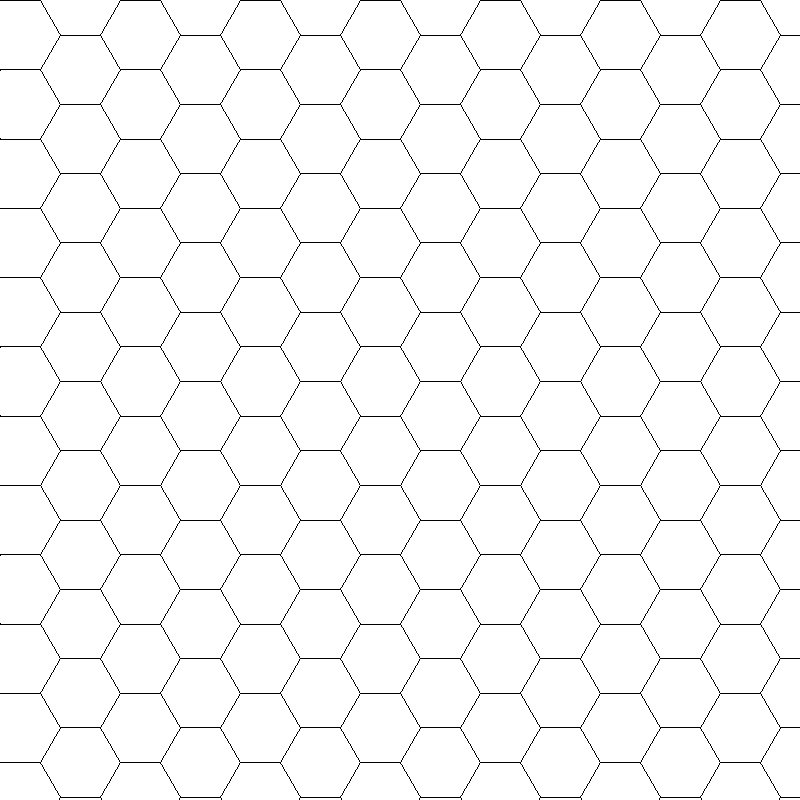
\includegraphics[width=55mm]{hexagon} & 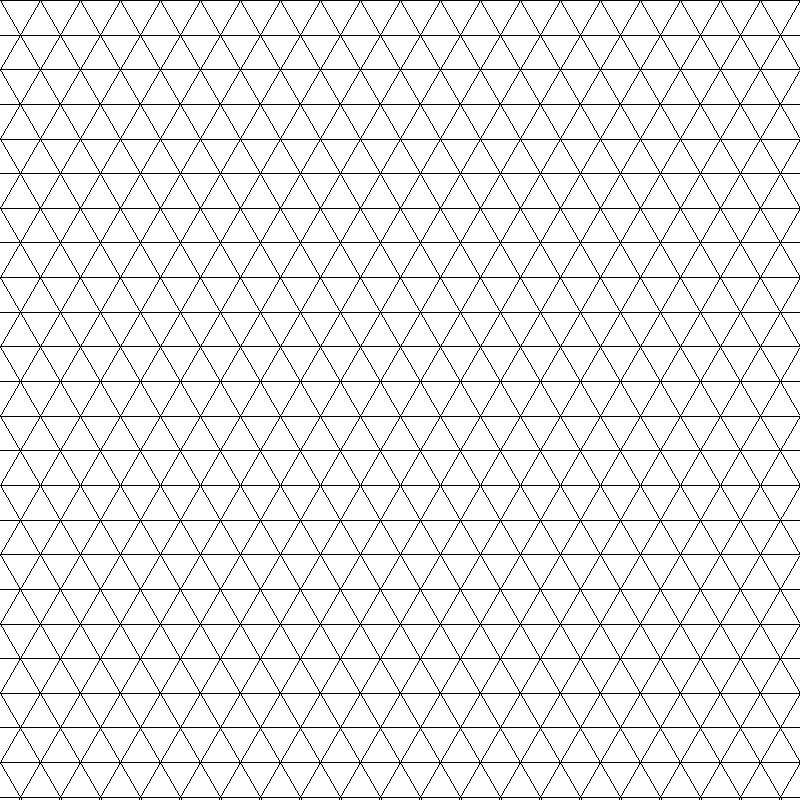
\includegraphics[width=55mm]{triangular} \\ Honeycomb
 & Triangular \\[6pt]
 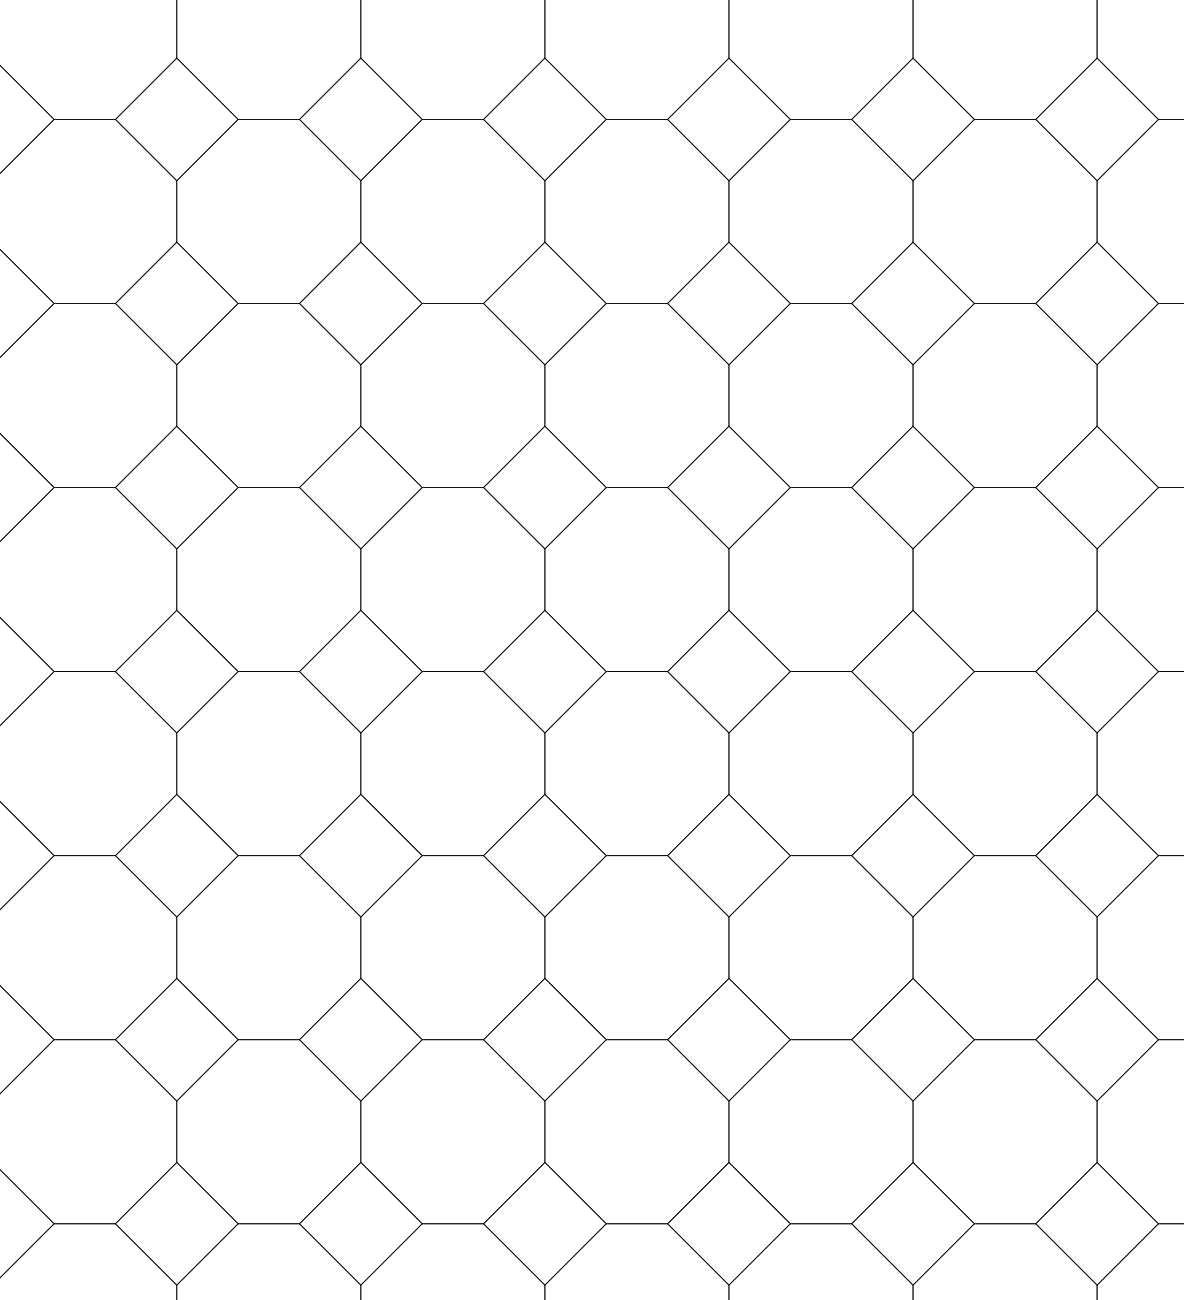
\includegraphics[width=
 55mm]{truncated_square_lattice} & 
\includegraphics[width=55mm]{lattice} \\
Truncated square & Square\\[2pt]
\end{tabular}
\label{fig:lattices}
\end{figure}

\subsection{Model}
Here we will see the basic model for bond percolation on any graph and then more specifically on a $\mathbb{Z}^d$ lattice. Thus, we have to define some basic tools in order to continue.

\paragraph{Self-avoiding path}
A self-avoiding path of length $n$ is a sequence of edges $e_1, ..., e_n$ such that $e_i = e_j \implies i = j$ and $e_i$ and $e_{(i + 1)}$ share an endpoint.

We call $\Omega_n$ the set of all of the self-avoiding paths of length $n$ that starts from the origin.

\paragraph{$\mathbb{Z}^d$ lattice}
Let us define $\mathbb{Z}^d=(\mathbb{V},\mathbb{E})$ where $\mathbb{V}=\mathbb{Z}^d$.
Two vertices $x$ and $y$ are connected by an edge $e \in \mathbb{E}$ if and only if $\sigma(x,y) = 1$ where
\[ \sigma(x,y) = \sum_{i = 1}^{d}{|x_i|+|y_i|}, \forall x, y \in \mathbb{Z}^d.\]

\begin{definition}[Bond percolation model]
Let $G = (V,E)$ be a graph with regularity (it ``looks'' the same from any vertex). We call bond percolation the process of opening a number of edges with a probability $\textit{p}\in [0,1]$. If an edge is not ``open'', we say it is ``closed''.
We consider the following space $(\Omega, \mathscr{F}, P_p)$ where
\begin{enumerate}[(i)]
  \item $\Omega = \{0,1\}^E,$
  
  \item  $\mathscr{F}$ is the $\sigma$-field of subsets of $\Omega$ generated by finite-dimensional cylinders,
  
  \item $P_p = \prod_{e \in E}{\mu_{e}}.$
  
We call $\omega \subset \Omega$ a percolation configurations where for $e \in E$

$$
\omega_e = \left\{
    \begin{array}{ll}
        0 & \mbox{if e is closed.}\\
        1 & \mbox{if e is open.}
    \end{array}
\right.
$$
\end{enumerate}
\end{definition}

\begin{definition}[$\mathbb{Z}^d$ bond percolation model]
For the lattice $\mathbb{Z}^d = (\mathbb{V}, \mathbb{E})$ defined above, we can study its bond percolation model associated $(\Omega, \mathscr{F}, \mathbb{P}_p)$ for a given $p \in [0,1]$ where for each $e\in\mathbb{E}$, $\mu_{e}$ is a Bernoulli measure of parameter $p\in [0,1]$.

\paragraph{}
Let $G = (V, E)$ be a planar graph. Its dual graph $G^*$ is the graph where for each face of $G$ we associate a unique vertex of $G^*$ such that two vertices of $G^*$ are connected by an edge when the two faces associated have an edge in common.

Let us define $(\mathbb{Z}^2)^*$ as the copy of $\mathbb{Z}^2$ translated by the vector $(\frac{1}{2}, \frac{1}{2})$ and for every configuration $\omega$ we associate the dual configuration $\omega^*$. And for every edge $e$ of $\mathbb{Z}^2$, let us define $e^*$ of $(\mathbb{Z}^2)^*$, as an edge intersecting $e$ in the middle. An edge of $(\mathbb{Z}^2)^*$ is open, if the edge associated in $\mathbb{Z}^2$ is closed. The law of $\omega^*$ is defined as a translate of $\mathbb{Z}^2$ by $(\frac{1}{2}, \frac{1}{2})$ of $\mathbb{P}_{1-p}$.

We can see this more clearly this in Figure \ref{fig:dual_graph}.

\begin{figure}
    \centering
    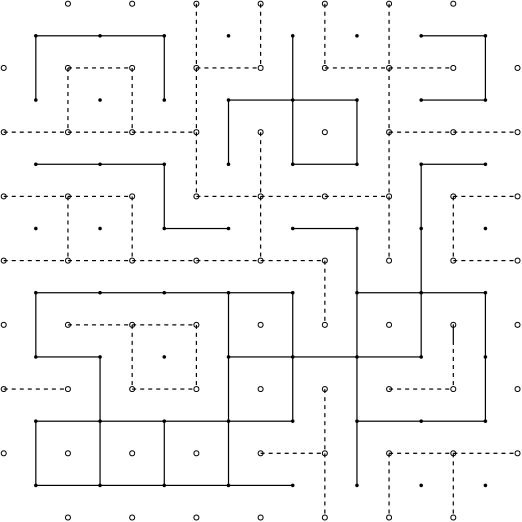
\includegraphics[scale=0.75]{dualgraph.png}
    \caption{Dual graph $\omega^* \subset (\mathbb{Z}^2)^*$ of $\omega \subset \mathbb{Z}^2$}
    \label{fig:dual_graph}
\end{figure}

\end{definition}

\subsubsection{$\mathbb{Z}^d$ Bernoulli percolation model}
At this point, the bond percolation on $\mathbb{Z}^d$ will be our main focus.

\paragraph{Box}
Let us define the $n$-box
\begin{itemize}
    \item We call  $B_n(x) = x + [-n, n]^d$ the box of size $n$ centered at a given vertex $x$ and $V_n(x)$ the vertices contained in $B_n(x)$ and $E_n(x)$ the edges contained in $B_n(x)$.
    \item We call $B_n = B_n(0)$ the box of size $n$ centered at $0$, and $V_n = V_n(0)$ the vertices contained in $B_n$ and $E_n = E_n(0)$ the edges contained in $B_n$.
\end{itemize}

\paragraph{Open path}
We call $\gamma$ a self-avoiding path a self-avoiding open path if and only if all of its edges are open in $\omega$.

\paragraph{Open edges}
We call $K(\omega)$ the subgraph of the open edges. An open cluster of a percolation configuration is a connected component of $K(\omega)$. The open cluster that contains a vertex $x \in V$ is denoted $C(x)$. If $x = 0$, we can denote $C = C(0)$ the open cluster that contains the origin.

\paragraph{}
Now let us define certain events related to the connection of two points or sets in $K(\omega)$.
\begin{itemize}
    \item If two vertices $x$ and $y$ of $G$ are connected by a self-avoiding open path, we write $x \longleftrightarrow y$ this event.
    \item If a vertex $x$ and a set of vertices $Y$ of $G$ that are connected by a self-avoiding open path, we write $x \longleftrightarrow Y$ this event.
    \item If two set of vertices $X$ and $Y$ of $G$ are connected by a self-avoiding open path, we write $X \longleftrightarrow Y$ this event.
    \item We say that $x$ is connected to $\infty$, when for every $n \geq 1$, there exists a self-avoiding open path of length $n$ and we write $x \longleftrightarrow \infty$ this event.
\end{itemize}

\paragraph{Infinite cluster}
An infinite cluster is an open cluster of an infinite size. We denote $|C|=\infty$. Alternatively, we can define an infinite cluster as an open cluster which contains arbitrarily large self-avoiding open paths. 

As we said earlier, our goal is to study the behavior of infinite open clusters depending on the parameter $p \in [0,1]$. Thus, let us define the functions $\theta : [0,1] \longrightarrow [0,1]$ the probability of an infinite cluster at zero and $\Phi : [0,1] \longrightarrow [0,1]$ the probability of the existence of an infinite cluster.

\begin{definition}[Probability of an infinite cluster at zero]
We will be interested in the probability that an infinite cluster at the origin exists.
Let us define
\[\theta(p) = P_p[0 \longleftrightarrow \infty] = P_p[|C|=\infty].\]
\end{definition}

\begin{remark}
Studying this probability for every $x \in \mathbb{V}$ is useless since as we said earlier, the graph ``looks'' the same from any vertex and the distribution of edges does not depend on a given vertex. Thus, we just have to study it for $x = 0$, the rest follows.
\end{remark}

\begin{definition}[Probability of an infinite cluster]
Let us define $\Phi(p)$ as :
\[ \Phi(p) = \mathbb{P}_p[\exists x \in \mathbb{V} : |C(x)| = \infty]. \]
which is the probability that an infinite cluster exists for a given $p \in [0,1]$.
\end{definition}

As we will see, there exists a critical probability $p_c$ where for $p < p_c$, there is no infinite cluster at $0$ almost surely.

\begin{definition}[Critical probability]
Let us define the critical probability $p_c$ as :
\[p_c = \sup\{p \ | \ \theta(p)=0\}.\]
\end{definition}

\paragraph{Boundary of a subgraph}
For a subgraph $S \subset \mathbb{Z}^d$, let us define the boundary of $S$ as

\[ \partial S = \{x \in V : \exists y \in \mathbb{Z}^d \text{ such that } xy \in \mathbb{E}\backslash E\}.\]
And the edge boundary as
\[ \Delta S = \{xy \in \mathbb{E}, x \in S, y \not\in S\}. \]

\begin{remark}
\text{}
\begin{enumerate}[(i)]
\item In $\mathbb{Z}^d$, for $\omega$, $x$ is connected to $\infty$ if and only if

\[ \forall n \in \mathbb{N}, x \longleftrightarrow \partial B_n(x). \]
\item \[ \lim_{n \rightarrow \infty}{\mathbb{P}_p[x \longleftrightarrow \partial B_n(x)]} = \mathbb{P}_p[x \longleftrightarrow \infty] = \mathbb{P}_p[|C(x)| = \infty].\]
\end{enumerate}
\end{remark}

\subsection{Formulas on events}
In this section, we will see some formulas related to the events of a Bernoulli bond percolation on the $\mathbb{Z}^d$ lattice that are crucial to understand the problem.
\subsubsection{Increasing events}
\paragraph{Increasing events}
\begin{itemize}
    \item We can put a partial order $\leq$ on $(\Omega, \mathscr{F})$ such that for two percolation configurations $\omega, \omega' \in \{0,1\}^\mathbb{E}$, we have
    \[ \omega \leq \omega' \Longleftrightarrow \forall e \in \mathbb{E}, \omega_e \leq \omega'_e. \]

    \item A random variable $X : \Omega \longrightarrow \mathbb{R}$ is said to be increasing if
    \[ \forall \omega, \omega' \in \{0,1\}^\mathbb{E}, \omega \leq \omega' \implies X(\omega) \leq X(\omega'). \]
    
    \item A random variable $X : \Omega \longrightarrow \mathbb{R}$ is said to be decreasing if $-X$ is increasing.
    
    \item An event $A$ is said to be increasing if $\mathbf{1}_A$ is increasing.
    
    \item Alternatively, an event $A$ is said to be increasing if
    \[ \forall \omega, \omega' \in \{0,1\}^\mathbb{E}, \omega \leq \omega' \text{ and }  \omega \in A \implies \omega' \in A. \]
    
    \item An event $A$ is said to be decreasing if $A^c$ is increasing.
\end{itemize}

\begin{proposition}
\label{increvent_prop}
  The event $A = \{ |C|=\infty \}$ is an increasing event.
\end{proposition}
\begin{proof}
Let us prove that $A = \{ |C|=\infty \}$ is an increasing event.
Suppose we have $\omega, \omega'$ two percolation configurations, such that $\omega \leq \omega'$. We call $C_\omega$ the cluster at the origin for $\omega$ and $C_{\omega'}$ the cluster at the origin for $\omega'$.
Because $\omega \leq \omega'$, it stands $C_{\omega} \subset C_{\omega'}$. Therefore $|C_{\omega}| = \infty \implies |C_{\omega'}| = \infty$, which means that $A$ is an increasing event.
\end{proof}

\begin{definition}[Increasing coupling]
Let $X$ be a random variable such that $X = (X_e), \: \forall e \in \mathbb{E}$ where all $X_e$ are uniform random variables on $[0,1]$.
For $p \in [0,1]$, we say

\[
\omega_p(e) = \left\{
    \begin{array}{ll}
        0 & \text{if $X_e < p$}.\\
        1 & \text{otherwise}.
    \end{array}
\right.
\]

We see that the law of $\omega_p$ is $\mathbb{P}_p$. Each edge is open with probability $p$, closed with probability $1- p$.
Fix $p < p'$, we can now define a measure $\mathbf{P}$ on $[0, 1] \longrightarrow \{0,1\}^{\mathbb{Z}^d}$ as the law of $p \longrightarrow \omega_p$ with marginals $\mathbb{P}_p$ such that

\[ \mathbf{P}[(\omega_p, \omega_{p'}) : \omega_p \leq \omega_{p'}] = 1. \]

\end{definition}

To prove Theorem \ref{increasingevent_theorem}, we will use increasing coupling. This will lead to the conclusion that $\theta$ is an increasing funcion since Proposition \ref{increvent_prop}.

\begin{theorem}
\label{increasingevent_theorem}
  If $A$ is an increasing event, then $p \longrightarrow \mathbb{P}_p[A]$ is an increasing function.
\end{theorem}
\begin{proof}
Since A is an increasing event, we have that :

\[ \omega_p \leq \omega_{p'} \implies (\omega_p \in A \implies \omega_{p'} \in A). \]

Thus,

\[ \mathbb{P}_p[A] = \mathbf{P}[\omega_p \in A] \leq \mathbf{P}[\omega_{p'} \in A] = \mathbb{P}_{p'}[A]. \]

\end{proof}

\begin{corollary}
  The function $\theta : [0,1] \longrightarrow [0,1]$ is increasing.
\end{corollary}
\begin{proof}
The event $A = \{ |C| = \infty \}$ is an increasing event. Therefore by applying Theorem \ref{increasingevent_theorem}, we deduce that the function $\theta(p) = \mathbb{P}_p[|C| = \infty]$ is increasing.
\end{proof}

This last result is important for the study of the critical phenomena that we will see in Section \ref{phasetransition_section} and justifies the existence of $p_c$ and of a phase transition. Furthermore, it implies that

\[
\left\{
    \begin{array}{ll}
        \theta(p) = 0 & \text{if $p < p_c$}.\\
        \theta(p) > 0 & \text{if $p > p_c$}.
    \end{array}
\right.
\]

\subsubsection{Harris' inequality}

Here are two first important inequalities.
\begin{proposition}[Harris' inequality]

\begin{enumerate}[(i)]
\text{}
\item If $A$ and $B$ are two increasing events, then

\[ \mathbb{P}_p[A \cap B] \geq \mathbb{P}_p[A]\mathbb{P}_p[B]. \]

\item If $X$ and $Y$ are two bounded increasing random variables, then
\[ \mathbb{E}_p[XY] \geq \mathbb{E}_p[X]\mathbb{E}_p[Y]. \]
\end{enumerate}
\end{proposition}

\begin{proof}
\text{}
\begin{enumerate}[(i)]
    \item (i) is implied by (ii) by setting $X = \mathbf{1}_A$ and $Y = \mathbf{1}_B$
    \item
    {
    First, let us prove by induction that
    
    \[ \forall f, g : \{ 0,1 \}^n \longrightarrow \mathbb{R} \text{ increasing functions} \]
    \[\mathbb{E}_p[f(\omega_1, ..., \omega_n)g(\omega_1, ..., \omega_n)] \geq \mathbb{E}_p[f(\omega_1, ..., \omega_n)]\mathbb{E}_p[g(\omega_1, ..., \omega_n)]. \]

        \paragraph{(Base case) (n=1)}
        
        Let $f, g : \{ 0,1 \} \longrightarrow \mathbb{R}$ be two increasing functions. Because adding a constant to $f$ or to $g$ does not change the inequality, we can assume that $f(0) = g(0) = 0$.
        Therefore, $f(1) \geq 0$ and $g(1) \geq 0$ since $f$ and $g$ are increasing.
        
        Thus,
        
        \begin{align*}
            \mathbb{E}_p[f(\omega_1)g(\omega_1)]-\mathbb{E}_p[f(\omega_1)]\mathbb{E}_p[g(\omega_1)] &= p f(1) g(1) - p^2 f(1) g(1) \geq 0.
        \end{align*}
        
        \paragraph{(Induction step)}
        Let $n \geq 1$ be a given integer and suppose that the hypothesis is true for this given $n$. We want to prove that it implies that it is true for $n + 1$.
                
        Let $f, g : \{ 0,1 \}^{n + 1} \longrightarrow \mathbb{R}$ be two increasing functions.
        We have
        \begin{align}
            \mathbb{E}_p[f(\omega_1,...,\omega_n,\omega_{n + 1})g(\omega_1,...,\omega_n,\omega_{n + 1})] &= 
            p \mathbb{E}_p[f(\omega_1,...,\omega_n,1)g(\omega_1,...,\omega_n,1) \nonumber \\  
            &+ (1 - p) \mathbb{E}_p[f(\omega_1,...,\omega_n,0)g(\omega_1,...,\omega_n,0)] \nonumber \\
            &\geq 
            p \mathbb{E}_p[f(\omega_1,...,\omega_n,1)]\mathbb{E}_p[g(\omega_1,...,\omega_n,1)] \nonumber \\
            &+ (1 - p) \mathbb{E}_p[f(\omega_1,...,\omega_n,0)]\mathbb{E}_p[g(\omega_1,...,\omega_n,0)] \nonumber \\
            &= p f_1(1) g_1(1) + (1 - p) f_1(0) g_1(0) \nonumber \\
            &= \mathbb{E}_p[f_1(\omega_{1})g_1(\omega_{1})] \nonumber \\ 
            &\geq \mathbb{E}_p[f_1(\omega_{1})]\mathbb{E}_p[g_1(\omega_{1})]. \label{eq:inequa_rec}
        \end{align}

        That proves the induction step, 
        \begin{align*}
        \mathbb{E}_p[f_1(\omega_{1})] &= p f_1(1) + (1-p) f_1(0) \\
        &= p \mathbb{E}_p[f(\omega_1, ..., \omega_n, 1)] + (1 - p) \mathbb{E}_p[f(\omega_1, ..., \omega_n, 0)] \\
        &= \mathbb{E}_p[f(\omega_1, ..., \omega_{n + 1})]. \\
        \mathbb{E}_p[g_1(\omega_{1})] &= \mathbb{E}_p[g(\omega_1, ..., \omega_{n + 1})].
        \end{align*}
        
        \paragraph{(Conclusion)}
        $\forall n \in \mathbb{N}$, all functions $f, g : \{ 0, 1 \}^n \longrightarrow \mathbb{R}$ increasing, then 
        
        \[\mathbb{E}_p[fg] \geq \mathbb{E}_p[f]\mathbb{E}_p[g].\]

    Let $X : \{ 0, 1 \} ^ \mathbb{E} \longrightarrow  \mathbb{R}$ and $Y : \{ 0, 1 \} ^ \mathbb{E} \longrightarrow  \mathbb{R}$ be two increasing bounded random variables. Let use define for all $n \geq 1$
    \[X_n = \mathbb{E}_p[X | \omega_1, \omega_2, ..., \omega_n]\]
    \[Y_n = \mathbb{E}_p[Y | \omega_1, \omega_2, ..., \omega_n]\]
    For every $n \geq 1$, we have
    \[\mathbb{E}_p[X_n Y_n] \geq \mathbb{E}_p[X_n] \mathbb{E}_p[Y_n]\]
    By applying the martingale convergence theorem, we obtain
    \[X_n \longrightarrow X \text{ and } Y_n \longrightarrow Y \text{ in } L^2. \]
    Thus by letting $n$ tend to $\infty$, we obtain
    \[\mathbb{E}_p[XY] \geq \mathbb{E}_p[X] \mathbb{E}_p[Y]\]
    }
\end{enumerate}
\end{proof}

\paragraph{Witness}
Let $A$ be an event. We say that $I \subset E$ is a witness of $A$ for $\omega$ if $\omega \in A$ and any configuration $\omega'$ coinciding with $\omega$ on $I$ belongs to $A$.

We say that $A$ and $B$ are realised disjointly if there exists two witnesses $I$ and $J$ for $\omega$ of $A$ (resp. $B$) that are disjoint.
We write this event as $A \circ B$.\\
Formally
\[ A \circ B = \{\omega \in \{ 0, 1 \}^\mathbb{N} : \exists I, J \text{ witnesses of } A \text{ (resp. B) in } \omega \text{ such that } I \cap J = \varnothing \}. \]

\paragraph{Example}
Here is an example of such events. Let $x,y,z,w$ be four different vertices of $\mathbb{Z}^d$ and $A$ be the event such that
    \[A = \{x \longleftrightarrow y\}\] and $B$ such that
    \[B = \{z \longleftrightarrow w\}.\]
We can see that $A \circ B$ is realised when $x$ and $y$ are connected by a self-avoiding open path $\gamma$ and $z$ and $w$ are connected by a self-avoiding open path $\Tilde{\gamma}$ such that $\gamma$ and $\Tilde{\gamma}$ are disjoints.

Here is the second most important inequality.
\begin{proposition}[BK-Reimer's inequality]
\label{bkreimer}
If $A$ and $B$ are two increasing events depending only on finitely many edges then
\[ \mathbb{P}_p[A \circ B] \leq \mathbb{P}_p[A]\mathbb{P}_p[B]. \]

\end{proposition}

\begin{remark}
The theorem is true for any event $A$ and $B$ depending only on finitely many edges. However, the proof was made by David Reimer and is too complex for this memoir. Therefore, the proof is left to the reader.

\end{remark}
\begin{proof}[Proof of proposition \ref{bkreimer}]
Let $A, B \subset \{0, 1\}^E$ be two increasing events depending only on a finite set of edges $E = \{ e_1, e_2, ... e_n \}$. We create a construction where all edges of $E$ are duplicated in one edge $e_i$ and one edge $e'_i$.

We assume that the witnesses of $A$ and $B$ are always opened.

We define the two copies of the space
\[ \omega_i = \omega(e_i). \]
\[\omega'_i = \omega(e'_i).\]
\[\omega = (\omega_1, ..., \omega_n).\]
\[\omega' = (\omega'_1, ..., \omega'_n).\]

We write $\overline{E} = E \cup E'$, $\overline{\omega}=(\omega, \omega')$ and $\overline{P}_p$ the corresponding measure.

For all $i \in \{0, ..., n\}$, let $\omega^{(i)} = (\omega'_1, \omega'_2, ..., \omega'_i, \omega_{i + 1}, ..., \omega_{n})$ be the interpolation between $\omega$ and $\omega'$.

Let $\overline{A}_i = \{ \overline{\omega} : \omega^{(i)} \in A \}$ and $\overline{B} = \{ \overline{\omega} : \omega \in B \}$.

$\overline{A}_n$ and $\overline{B}$ being independents, we have

\[ \overline{\mathbb{P}}_p[\overline{A}_n \circ \overline{B}] = \overline{\mathbb{P}}_p[\overline{A}_n]\overline{\mathbb{P}}_p[B] = \mathbb{P}_p[A]\mathbb{P}_p[B]\]

since $\overline{A}_n$ and $\overline{B}$ depend only on disjoint set of edges.
And
\[ \overline{\mathbb{P}}_p[\overline{A}_0 \circ \overline{B}] = \mathbb{P}_p[A \circ B]\]
since $\overline{A}_0$ and $\overline{B}$ are defined only in term of $\omega$.

We can rewrite BK-Reimer's inequality as :
\[\mathbb{P}_p[A \circ B] = \mathbb{P}_p[\overline{A}_0 \circ \overline{B}] \leq \mathbb{P}_p[\overline{A}_n \circ \overline{B}] = \mathbb{P}_p[A]\mathbb{P}_p[B].\]

That means we just have to prove for every $i \in \{1, ..., n \}$ that
\[ \mathbb{P}_p[\overline{A}_{i - 1} \circ \overline{B}] \leq \mathbb{P}_p[\overline{A}_{i} \circ \overline{B}].\]

Let us decompose the event $\overline{A}_{i - 1} \circ \overline{B}$ in three different events
\[ C_1 = \{\exists I, J \subset \overline{E} \backslash \{e_i, e'_i\}, I, J \text{ disj.}, I \text{ wit. of } \overline{A}_{i - 1} \text{ and } J \text{ wit. of } \overline{B} \text{ for } \overline{\omega}\}. \]
\[ C_2 = C_1^c \cap \{\exists I, J \subset \overline{E} \backslash \{e_i, e'_i\}, I, J \text{ disj.}, I \text{ wit. of } \overline{A}_{i - 1} \text{ for } \overline{\omega} \text{ and } J\cup\{e_i\} \text{ wit. of } \overline{B} \text{ for } \overline{\omega}^{e_i}\}. \]
\[ C_3 = C_1^c \cap C_2^c \cap \{\exists I, J \subset \overline{E} \backslash \{e_i, e'_i\}, I \cap J = \varnothing, I\cup\{e_i\} \text{ wit. of } \overline{A}_{i - 1} \text{ for } \overline{\omega} \text{ and } J \text{ wit. of } \overline{B} \text{ for } \overline{\omega}^{e_i}\}. \]
We can observe that $C_1$, $C_2$ and $C_3$ are independent of $\omega_i$ and $\omega'_i$.
And

\[\overline{A}_{i - 1} \circ B = C_1 \sqcup (C_2 \cap \{\omega_i = 1\}) \sqcup (C_3 \cap \{\omega_i = 1\}) \subset \overline{A}_{i} \circ B.\]

Therefore,

\[\overline{\mathbb{P}}_p[\overline{A}_{i - 1} \circ B] = \overline{\mathbb{P}}_p[C_1] + p(\overline{\mathbb{P}}_p[C_2] + \overline{\mathbb{P}}_p[C_3]) \leq \mathbb{P}_p[\overline{A}_i \cap \overline{B}].\]

Which was what we wanted to prove.
\end{proof}

\begin{corollary}
If $S$ is a finite set containing $0$ and $x \not\in S$, then

\[ \mathbb{P}_p[0 \longleftrightarrow x] \leq \sum_{y \in \partial S}{\mathbb{P}_p[0 \stackrel{S}{\longleftrightarrow} y]\mathbb{P}_p[y \longleftrightarrow x]}. \]
\end{corollary}

\begin{proof}
Fix $n \geq 1$. If $0$ is connected to $x$ in $B_n$, there exists a self-avoiding path $\gamma$ of open edges of $B_n$ from $0$ to $x$. Let $y$ be the first vertex in $\partial S$ on the self-avoiding open path $\gamma$.

Thus,

\[ \mathbb{P}_p[0 \stackrel{B_n}{\longleftrightarrow} x] \leq \sum_{y \in \partial S}{\mathbb{P}_p[\{0 \stackrel{S}{\longleftrightarrow} y\} \circ \{y \stackrel{B_n}{\longleftrightarrow} x\}]}.\]

And by applying BK-Reimer's inequality (Theorem \ref{bkreimer}), we have

\[ \mathbb{P}_p[0 \stackrel{B_n}{\longleftrightarrow} x] \leq \sum_{y \in \partial S}{\mathbb{P}_p[0 \stackrel{S}{\longleftrightarrow} y]\mathbb{P}_p[y \stackrel{B_n}{\longleftrightarrow} x]}.\]

And by letting $n$ tend to $\infty$, we obtain what we wanted to prove.
\end{proof}

\subsubsection{Russo's formula}
Let us define the concept of pivotal points.
\paragraph{Pivotal point}
Set $\omega^{(e)}$ as the configuration coinciding with $\omega$ except at $e$, where it is equal to $1$ and $\omega_{(e)}$ the configuration coinciding with $\omega$ except at $e$, where it is equal to $0$.

We have that
\[ \omega \in \mathrm{Piv}_e(A) \Longleftrightarrow \omega^{(e)} \in A \text{ and } \omega_{(e)} \not\in A. \]

We say that $e$ is pivotal for $A$ when $\omega \in \mathrm{Piv}_e(A)$.

\begin{theorem}[Russo's formula]
\label{russo_formula}
If $A$ is an increasing event depending only on a finite number of edges, we have

\[ \frac{\partial }{\partial p}{\mathbb{P}_p[A]} = \sum_{e \in E}{\mathbb{P}_p[\mathrm{Piv}_e(A)]}. \]
\end{theorem}

\begin{proof}
Set $E = \{ e_1, ... e_k \}$.
$\forall p_1 ... p_k \in [0,1]$, we can define $\mathbb{P}_{p_1, ... p_k}$ as

\[ \mathbb{P}_{p_1, ... p_k}[\{\omega\}] = \prod_{i = 1}^{k}{p_{i}^{\omega_i} (1 - p_{i})^{1 - \omega_i}}, \space\forall \omega \in \{ 0,1 \}^E. \]

Let us define $f$ as $f(p_1, ..., p_k) = \mathbb{P}_{p_1, ..., p_k}[A]$.

We remark that $f(p, ..., p) = \mathbb{P}_{p}$.

Hence,

\[ \frac{\partial}{\partial p} \mathbb{P}_{p}[A] = \frac{\partial}{\partial p} \mathbb{P}_{p, ... ,p}[A] = \frac{\partial}{\partial p} f(p, ..., p) = \sum_{i = 1}^{k}{\frac{\partial}{\partial p_i}f(p, ... p)}. \]

Let us compute the right partial derivatives of $f$ (we can define the left partial derivatives analogically)

\[ \frac{\partial}
{\partial p_i}f(p, ..., p) = \lim_{\varepsilon \rightarrow 0 ; \varepsilon > 0}{\frac{f(p,...,\overbrace{p+\varepsilon}^{i\text{-th}},...,p) - f(p,...,p)}{\varepsilon}}. \]
for $i$ such that $1 \leq i \leq k$ and $p < 1$.

Let $U_1, ..., U_k$ be uniform random variables in $[0,1]$. For $q \in [0, 1]$, we define
\[
\omega_q(e_j) = \left\{
    \begin{array}{ll}
        \mathbf{1}_{U_j \leq p} & \text{if } i \not= j.\\
        \mathbf{1}_{U_i \leq q} & \text{if otherwise.}
    \end{array}
\right.
\]

Then,

\begin{align*}
f(p, ..., \overbrace{p+\varepsilon}^{i\text{-th}}, ..., p) - f(p, ... p) &= \mathbb{P}[\omega_{p + \varepsilon} \in A] - \mathbb{P}[\omega_{p} \in A] \\
&= \mathbb{P}[\omega_{p + \varepsilon} \in A \text{ and } \omega_{p} \not\in A] \\
&= \mathbb{P}[e_i \text{ is pivotal for } A \text{ in } \omega_p, U_i \in [p, p + \varepsilon]] \\
&= \varepsilon \mathbb{P}[e_i \text{ is pivotal for } A \text{ in } \omega_p] \\
\frac{f(p, ...,\overbrace{p+\varepsilon}^{i\text{-th}}, ..., p) - f(p, ... p)}{\varepsilon} &=\mathbb{P}[e_i \text{ is pivotal for } A \text{ in } \omega_p]. \\
\end{align*}

Thus,

\[ \frac{\partial}{\partial p_i}(p, ..., p) = \mathbb{P}_p[e_i \text{ is pivotal for } A].\]

Therefore,

\[ \frac{\partial}{\partial p} \mathbb{P}_{p}[A] = \sum_{i = 1}^{k}{\frac{\partial}{\partial p_i}f(p, ... p)} = \sum_{e \in E}{\mathbb{P}_p[\mathrm{Piv}_e(A)]}.\]
And that proves the point.
\end{proof}

\section{Phase transition of the Bernoulli percolation} \label{phasetransition_section}
Let us study the phase transition phenomena of the Bernoulli bond percolation on $\mathbb{Z}^d$ for $d \geq 1$. We divide the problem in two cases: one trivial case for $d = 1$ and another case for $d \geq 2$. We will see that $p_c \in [0,1]$ and given that $\theta$ is increasing, it confirms the critical phenomena.

\begin{theorem}[$d = 1$]
  If $d = 1$, then $p_c(d) = 1$.
  There is almost never an infinite cluster at $0$ if $p < 1$ and there is almost always an infinite cluster at $0$ if $p = 1$.
\end{theorem}

\begin{proof}

Let us study $\mathbb{Z}^1$ percolation. We know for sure that if $p < 1$ then almost certainly there exists a closed edge to the left of the origin, and another one closed to the right. Thus almost surely, there is no infinite cluster at $0$ if $p < 1$. If $p = 1$,  an infinite cluster at $0$ exists almost surely.

\begin{figure}[ht]
\centering
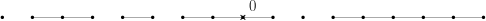
\includegraphics{Z1lattice}
\caption{Example of a percolation on the $\mathbb{Z}^1$ lattice, size = $17$, $p = 0.5$}
\end{figure}
\end{proof}

\begin{theorem}[$d \geq 2$ case]
  For all $d \geq 2$, $0 < p_c(d) < 1$.
\end{theorem}

\begin{proof}

First, we shall prove that $\forall d \geq 2$, $p_c(d) > 0$.

Saying that $C$ is an infinite cluster is equivalent to saying that there exists arbitrarily long self-avoiding open paths in $C$, which means that for every $n \geq 1$
\begin{align*} 
\theta(p) &\leq \mathbb{P}_p[ \text{there exists } \gamma \in \Omega_n  \text{ such that } \omega_e = 1  \text{ for every } e \in \gamma] \\
&\leq \sum_{\gamma \in \Omega_n} \mathbb{P}_p[\omega_e = 1 \text{ for every } e \in \gamma] && \text{ (the edges being independants)} \\
&\leq |\Omega_n|p^n \\
&\leq (2dp)^n. && (\text{because $|\Omega_n| \leq (2d)^n$})
\end{align*}

If we let this $n$ tend to $0$ when $p < \frac{1}{2d}$, the right quantity $(2dp)^n$ tends to zero, which implies that $\theta(p) = 0$.
That is to say, $p \leq p_c(d)$. Thus $\frac{1}{2d} \leq p_c(d)$.

Now let us show that $p_c(d) < 1$. We have to prove that when $p$ is close enough to $1$, $\theta(p) > 0$.

\paragraph{Case $d=2$.}
Saying that the origin is not in an infinite cluster in $\omega$ is the same as saying there exists a finite necklace of open edges in $\omega^*$ surrounding this cluster. We can see this more clearly in Figure \ref{fig:finiteneckl}.

Therefore,

\begin{align}
1 - \theta(p) &\leq \sum_{n \geq 1}{\mathbb{P}_p[\omega^* \text{ contains an open circuit surrounding 0 passing through $(n + 1/2, 0)$}}] \nonumber \\
 &\leq \sum_{n \geq 1}{\mathbb{P}_p[\omega^* \text{ contains an open path of length $2n+4$ passing through $(n + 1/2, 0)$}}] \nonumber \\
 &\leq \sum_{n \geq 1}{({4(1-p)})^{2n+1}}. \label{eq:ineq_finitneckl}
\end{align}
We obtain (\ref{eq:ineq_finitneckl}) because the probability of \[\{\omega^* \text{ contains an open path of length $2n+4$ passing through $(n + 1/2, 0)$}\}\]
is less than $(4(1-p))^{2n+4}$ because the probability that $2n+4$ edges of $\omega^*$ are open is $(1-p)^{2n+4}$ and there are less than $4^{2n+1}$ such paths.
When $p$ is close enough to $1$, the sum is strictly smaller than $1$, therefore $\theta(p) > 0$, thus $p_c(2) < 1$.

\begin{figure}
    \centering
    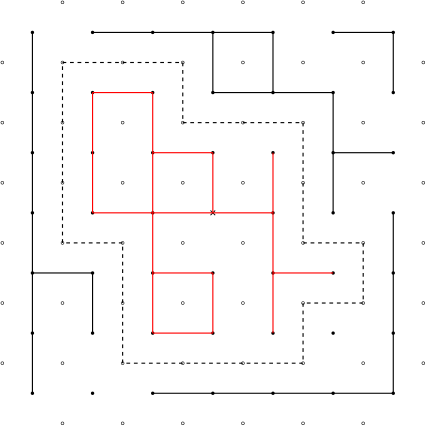
\includegraphics{finiteneckclace.png}
    \caption{Open circuit of $\omega^*$ (in dashed) surrounding the cluster at the origin (in red)}
    \label{fig:finiteneckl}
\end{figure}

\paragraph{Case $d > 2$.}
For $\mathbb{Z}^d$ with $d > 2$, we can see that $\mathbb{Z}^d$ contains a copy of $\mathbb{Z}^2$ containing $0$, thus if $0$ is connected to $\infty$ in $\mathbb{Z}^2$, then $0$ is connected to $\infty$ is in $\mathbb{Z}^d$, thus $p_c(d) \leq p_c(2) < 1$.

In conclusion we have
\[\forall d \geq 2, 0 < p_c(d) < 1.\]
And that concludes the proof.
\end{proof}

\subsection{Subcritical phase}

The subcritical phase is when $p < p_c$.
We will prove that if $p < p_c$, there is almost never an infinite open cluster, and furthermore that the diameter of an open cluster of a given vertex decays exponentially.

Let us define the probability $\theta_n$ that an open path from the origin is crossing the $n$-box as \[\theta_n(p)=\mathbb{P}_p[0 \longleftrightarrow \partial B_n].\]

We write $0 \stackrel{S}{\longleftrightarrow} x$ for saying that $0$ is connected to $x$ using the edges of a subgraph $S$.
And we define $\phi_p(S)$ as

\[ \phi_p(S) = p\sum_{xy \in \Delta S} \mathbb{P}_p[0 \stackrel{S}{\longleftrightarrow} x]. \]

\begin{remark}
$\phi_p$ can be seen as the average number of open edges $S$

\begin{align*}
    \phi_p(S) &= \sum_{xy \in \Delta S}{\mathbb{P}_p[xy \text{ is open}]\mathbb{P}_p[0 \stackrel{S}{\longleftrightarrow} x]} \\
    &= \sum_{xy \in \Delta S}{\mathbb{P}_p[xy \text{ is open}, 0 \stackrel{S}{\longleftrightarrow} x]} \\
    &= \mathbb{E}\left[\sum_{xy \in \Delta S}{\mathbf{1}_{0 \stackrel{S}{\longleftrightarrow} x, xy \text{ open}}}\right] \\
    &= \mathbb{E}[\text{``Number of open edges through which } S \text{ can exit starting at 0''}]. \\
\end{align*}
\end{remark}

Here are two lemmas that will be important in order to prove exponential decay (Theorem \ref{exponentialdecay}). First, we want to prove the exponential decay for a finite set $S$ such that $\phi(S) < 1$ (Lemma \ref{firstlemma_expdecay}). Then we will prove that it is in fact always the case for all $p < p_c$.
\begin{lemma}
\label{firstlemma_expdecay}
If there exists a finite set $S$ that contains the origin where $\phi_p(S) < 1$, then there exists a constant $c_p > 0$, such that
\[ \forall n \geq 1, \theta_n(p) \leq \exp(-c_p n). \]
\end{lemma}

\begin{proof}
Choose $L$ such that $S \subset B_L$. If $0 \longleftrightarrow B_{L n}$ occurs (let $\gamma$ be the self-avoinding open path), then there exists an edge at the boundary of $S$ such that $\{0 \longleftrightarrow x \text{ and } xy  \text{ is open}\}$ and $\{y \longleftrightarrow \partial B_{L n}\}$ occurs disjointly. We consider the piece of the open path $\gamma$ from $0$ to the first vertex $y \in \partial S$ as witness for the first event and the other piece as witness for the second event.

If we apply the BK-Reimer's inequality (Theorem \ref{bkreimer}), we obtain
\begin{align*}
    \mathbb{P}_p[0 \longleftrightarrow \partial B_{Ln}] &\leq \sum_{xy \in \Delta S}{\mathbb{P}_p[\{0 \stackrel{S}{\longleftrightarrow}, xy \text{ is open}\}\circ\{y \longleftrightarrow \partial B_{L n}\}]} \\
    &\leq \sum_{xy \in \Delta S}{\mathbb{P}_p[\{0 \stackrel{S}{\longleftrightarrow} x, xy \text{ is open}\}]\mathbb{P}_p[\{y \longleftrightarrow \partial B_{L n}\}]} \\
    &\leq \phi_p(S) \mathbb{P}_p[0 \longleftrightarrow \partial B_{L (n - 1)}]. \\
\end{align*}

By induction, we have $\forall n \geq 1$
\[ \mathbb{P}_p[0 \longleftrightarrow \partial B_{L n}] \leq \phi_p(S)^n.\]
And that proves the exponential decay.
\end{proof}

\begin{lemma} 
\label{secondlemma_expdecay}
For all $n \geq 1$, $\mathbf{S} = \{z \in B_n : z \not\leftrightarrow \partial B_n \}$ is the set of points that are not connected to the boundary of the $n$-box.

For all $p \in (0, 1)$, we have
\[ \theta_n'(p)=\frac{1}{p(1-p)}\mathbb{E}_p[\phi_p(\mathbf{S})]. \]
\end{lemma}

\begin{proof}
$\{0 \longleftrightarrow \partial B_n\}$ is an increasing event depending only on finitely many edges. By applying Russo's formula (Theorem \ref{russo_formula}) to $\{0 \longleftrightarrow \partial B_n\}$, we have

\begin{align} 
\theta_n'(p) = \frac{\partial}{\partial p}{\mathbb{P}_p[0 \longleftrightarrow \infty]} &= \sum_{e \in E_n}\mathbb{P}_p[e \text{ is pivotal for } 0 \longleftrightarrow \partial B_n] \nonumber \\
 &= \frac{1}{1 - p} \sum_{e \in E_n}\mathbb{P}_p[\omega_e = 0 \text{ and } e \text{ is pivotal for } 0 \longleftrightarrow \partial B_n] \label{eq:der_theta_n}
\end{align}

We obtain the equality (\ref{eq:der_theta_n}) because the events $\{e$ is pivotal for $0 \longleftrightarrow \partial B_n\}$ are all independents of $\omega_e$.

There we can observe that an edge $e$ is pivotal for $\{ 0 \longleftrightarrow \partial B_n \}$ if and only if

\begin{enumerate}[(1)]
\item One of the extremity $x$ is connected to $0$,
\item The other extremity $y$ is connected to $\partial B_n$,
\item $0$ is not connected to $\partial B_n$.
\end{enumerate}

Which means that :

\begin{align*}
\theta_n'(p) &= \frac{1}{1 - p}\sum_{x,y \in B_n, xy \in E_n}{\mathbb{P}_p[0 \leftrightarrow x, y \leftrightarrow \partial B_n, 0 \not\leftrightarrow \partial B_n]} \\
&= \frac{1}{1 - p} \sum_{S \subset B_n}{\sum_{xy \in \Delta S}{\mathbb{P}_p[0 \stackrel{S}{\longleftrightarrow} x, \textbf{S} = S]}} \\
&= \frac{1}{1 - p}\sum_{S \subset B_n}{\sum_{xy \in \Delta S}{\mathbb{P}_p[0 \stackrel{S}{\longleftrightarrow} x]}} \mathbb{P}_p[\mathbf{S} = S] \\
&= \frac{1}{1 - p}\mathbb{E}_p\left[\frac{1}{p}\phi_p(S)\right] \\
&= \frac{1}{p(1 - p)}\mathbb{E}_p[\phi_p(S)].
\end{align*}
And that concludes the proof.
\end{proof}

Now that we have proved the two lemmas, we can attack the exponential decay.
\begin{theorem}[Exponential decay]
\label{exponentialdecay}
  Fix $d \geq 2$, for all $p < p_c(d)$, there exists a constant $c_p$ such as for all $n \geq 1$
  \[ \mathbb{P}_p(0 \longleftrightarrow \partial B_n) \leq exp(-c_p n). \]
  Furthermore, there exists $c > 0$ such that for all $p > p_c$
  \[\theta(p) \geq c(p - p_c).\]
\end{theorem}

\begin{proof}
We want to prove that for all $p < p_c$, there exists $S \subset \mathbb{Z}^d$ such that $\phi_p(S) < 1$.

Let us set $\Tilde{p}_c$ as
\[ \Tilde{p}_c = \sup\{p \in [0,1] : \exists S \text{ a finite set that contains zero such that } \phi_p(S) < 1\}. \]

Using Lemma \ref{firstlemma_expdecay}, we have that for any $p < \Tilde{p}_c$, there exists a constant $c_p > 0$ such that $\forall n \geq 1, \theta_n(p) \leq \exp(-c_p n)$

Since $\theta_n(p) \xrightarrow[n \rightarrow \infty]{} \theta(p)$, we have $\theta(p) = 0$ and $p \leq p_c$. Thus, we obtain $\Tilde{p}_c \leq p_c$.

Now, let us prove that $\Tilde{p}_c \geq p_c$, which is the same as $\theta(p) > 0 \text{ for all } p > \Tilde{p}_c$. Fix $p > \Tilde{p}_c$ such that $\phi_p(S) \geq 1$ for all S that contains $0$, and $\phi_p(S) = 0$ for all S that does not contain $0$.

Using Lemma \ref{secondlemma_expdecay} we obtain

\begin{align*}
    \theta'_n(p) &= \frac{1}{p(1-p)}\mathbb{E}_p[\phi_p(S)] \\
    &\geq  \frac{1}{p(1-p)}\mathbb{E}_p[0 \in \mathbf{S}] \\
    &= \frac{1}{p(1-p)}(1-\theta_n(p)).
\end{align*}

That is to say  

\[ \left[\log\left(\frac{1}{1-\theta_n}\right)\right]' \geq \left[\log\left(\frac{p}{1-p}\right)\right]'.\]
By integrating between $\Tilde{p}_c$ and $p$,
\[ \log\left(\frac{1}{1 - \theta_n(p)}\right) - \log\left(\frac{1}{1 - \theta_n(\Tilde{p}_c)}\right) \geq \log\left(\frac{p}{1-p}\right) -\log\left(\frac{\Tilde{p}_c}{1-\Tilde{p}_c}\right). \]
\[ \log\left(\frac{1 - \theta_n(\Tilde{p}_c)}{1 - \theta_n(p)}\right) \geq \log\left(\frac{p(1 - \Tilde{p}_c)}{(1-p)\Tilde{p}_c}\right). \]
Because $\log$ is an increasing function
\[ \frac{1}{1 - \theta_n(p)} \geq \frac{1 - \theta_n(\Tilde{p}_c)}{1 - \theta_n(p)} \geq \frac{p(1 - \Tilde{p}_c)}{(1-p)\Tilde{p}_c}. \]
Because $x \longrightarrow 1/x$ is a decreasing function in $\mathbb{R}_+$
\[ 1 - \theta_n(p) \leq \frac{(1-p)\Tilde{p}_c}{p(1 - \Tilde{p}_c)}. \]
By rearranging  the terms
\[ \theta_n(p) \geq \frac{p - \Tilde{p}_c}{p(1 - \Tilde{p}_c)}. \]
Now, if we let $n$ tend to $\infty$, we have
\[ \theta(p) \geq \frac{p - \Tilde{p}_c}{p(1 - \Tilde{p}_c)} > 0. \]

Thus, $p_c = \Tilde{p_c}$, which means by the definition of $\Tilde{p_c}$ that for all $p < p_c = \Tilde{p_c}$, there exists a finite set $S$ such that $\phi_p(S) < 1$, and by using the Lemma \ref{firstlemma_expdecay}, it implies that for all $n \geq 1$, there exists $c_p > 0$ such that

\[ \forall n \geq 1, \mathbb{P}_p(0 \longleftrightarrow \partial B_n) \leq \exp(-c_p n). \]
This concludes the point.
\end{proof}

\subsection{Ergodicity}

In order to prove that there exists an infinite cluster almost surely for all $p > p_c$ (Theorem \ref{ergodicity_pp}), we will use the ergodicity of $\mathbb{P}_p$.

Let $\tau_x$ be a translation by a vector $x \in \mathbb{Z}^d$. We have
\begin{enumerate}[(1)]
    \item $\tau_x A = \{ \omega \in \{0,1\}^\mathbb{E} : \tau_x^{-1}\omega \in A \}$,
    \item An event $A$ is called invariant under translations if $\forall x \in \mathbb{Z}^d$, $\tau_{x}A=A$,
    \item The measure $\mu$ is said to be invariant under translations if $\mu(\tau_x A) = \mu(A)$  for any event $A$ and any $x \in \mathbb{Z}^d$.
\end{enumerate}
    
\begin{definition}[Ergodicity]
The measure $\mu$ is said to be ergodic if for any event $A$ invariant under translations, $\mu(A) \in \{0,1\}.$
\end{definition}

\begin{theorem}[Ergodicity of the measure of $\mathbb{Z}^d$]
\label{ergodicity_pp}
The measure $\mathbb{P}_p$ is invariant under translations. Moreover, the measure $\mathbb{P}_p$ is ergodic.
\end{theorem}

\begin{proof}
First, let us prove that the measure $\mathbb{P}_p$ is invariant under translations. Let $A$ be an event depending only on a finite number of edges, and $x$ a vector in $\mathbb{Z}^d$.
We have that

\[\mathbb{P}_p[A] = \mathbb{P}_p[\tau_x A]. \]

Because this property is true for all increasing events depending only on a finite number of edges and that these events generate the set of all events, $\mathbb{P}_p$ is invariant under translations.

Second, let us show that the measure $\mathbb{P}_p$ is ergodic. Let $A$ be an event invariant under translations. 
We will prove that
\[ \mathbb{P}_p[A]\in \{0,1\}.\]

Let us prove that $\mathbb{P}_p[A] \leq \mathbb{P}_p[A]^2$. Fix $\varepsilon > 0$. We know for sure that $A$ is the limit of a sequence of events $(A_n)_{n \in \mathbb{N}}$ depending only on a finite number of edges. We can choose an event $B$ of this sequence that depends only on a finite number of edges such that $\mathbb{P}_p[A \Delta B] \leq \varepsilon$ where $A \Delta B = (A\backslash B) \cup (B \backslash A)$.

Because $B$ depends only on a finite set $E$ of edges, there exists a vector $x$ large enough so that $\tau_x E \cap E = \varnothing$. Therefore $B$ and $\tau_x B$ are independents and
\begin{align*}
    \mathbb{P}_p[B \cap \tau_x B] &= \mathbb{P}_p[B]\mathbb{P}_p[\tau_x B] \\
    &=\mathbb{P}_p[B]^2. && \text{(invariance under translation)}
\end{align*}

Thus,

\begin{align*}
    \mathbb{P}_p[A] &= \mathbb{P}_p[A \cap A] \\
    &= \mathbb{P}_p[A \cap \tau_x A] \\
    &\leq \mathbb{P}_p[B \cap \tau_x B] + 2\varepsilon \\
    &= \mathbb{P}_p[B]^2 + 2\varepsilon \\
    &\leq \mathbb{P}_p[A]^2 + 4\varepsilon.
\end{align*}

Taking the limit of the inequality when $\varepsilon$ tends to zero, we have
$\mathbb{P}_p[A] \leq \mathbb{P}_p[A]^2$. Therefore, $\mathbb{P}_p[A] \in \{0, 1\}$.
This concludes the proof.
\end{proof}

\begin{corollary}
If $p > p_c$, then there exists an infinite open cluster almost surely.
\end{corollary}
\begin{proof}
The event
\[A = \{\exists x \in \mathbb{V} : |C(x)| = \infty\}\] 
is invariant under translation. Thus,
\[\mathbb{P}_p[A] \in \{0,1\}.\]
Since $\theta(p) > 0$, we have $\mathbb{P}_p[A] = 1$. There exists an infinite open cluster almost surely.
\end{proof}

\subsection{Uniqueness of the infinite cluster}
We will see that when $p > p_c$ not only there exists an infinite cluster almost surely but also this infinite cluster is unique almost surely. We have to define what we call a trifurcation which will be a useful tool to prove the uniqueness of the infinite cluster (Theorem \ref{unique_infcluster}).
\paragraph{Trifurcation}
Let $\omega \in \{ 0, 1 \}^d$ be a percolation configuration. A vertex $x$ is called a trifurcation in $\omega$ if
\begin{enumerate}[(i)]
\item $x$ has exactly three adjacent edges.
\item $C(x)$ splits into three different infinite clusters $C_1$, $C_2$, $C_3$ if we close the edges adjacent to $x$.
\end{enumerate}
A trifurcation $x$ is represented in Figure \ref{fig:trif}.

We define the event
\[\mathscr{T}_x = \{x \text{ is a trifurcation}\}.\]

\begin{figure}
    \centering
    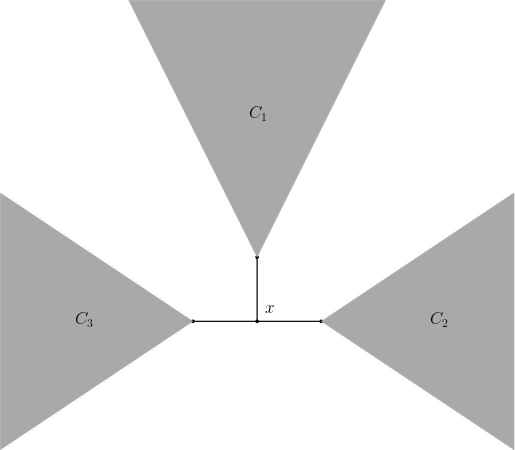
\includegraphics[scale=0.35]{trif.png}
    \caption{A trifurcation $x$, the three clusters are represented by gray triangles.}
    \label{fig:trif}
\end{figure}

\begin{remark}
$x \in \mathbb{Z}^d$ is a trifurcation if and only if $\tau_x \mathscr{T}_0 = \mathscr{T}_x$.
\end{remark}

\begin{theorem}[Uniqueness of the infinite cluster]
\label{unique_infcluster}
For all $p \in [0,1]$ such that $\theta(p) > 0$,
\[\mathbb{P}_p[\exists! \text{ infinite cluster}] = 1.\]
\end{theorem}

\begin{proof}
Assume that $p \in (0,1)$, $p = 0$ and $p = 1$ being trivial. Let us write $N$ as the random variable of the number of infinite open clusters in $\mathbb{Z}^d$.
We can rewrite the theorem as follows

For every $p \in (0, 1)$
\[ \mathbb{P}_p[N = 0] = 1 \text{ or } \mathbb{P}_p[N = 1] = 1.\]

$\mathbb{P}_p$ being ergodic, $\forall k \in \mathbb{N}$, $\mathbb{P}_p[N = k] = 0$ or $\mathbb{P}_p[N = k] = 1$.
Furthermore,

\[ \mathbb{P}_p\left[\bigcup_{0 \leq k \leq \infty}{\{N = k\}}\right] =  \sum_{0 \leq k \leq \infty}{\mathbb{P}_p[N = k]} = 1.\]

Hence, there is one and only $k \in \mathbb{N} \cup \{ \infty \}$ such that $\mathbb{P}_p[N = k] = 1$.

First we want to prove that $k \in \{0, 1, \infty\}$.

Suppose that $1 < k < \infty$.
Let $\mathscr{F}_n$ be an event such that

\[ \mathscr{F}_n = \{B_n \longleftrightarrow \infty \text{ and all infinite clusters intersect } B_n \}. \]
If we choose $n$ large enough, we have $\mathbb{P}_p[\mathscr{F}_n] \geq \frac{1}{2}$ since $1 < N < \infty$ almost surely.

\begin{align*}
\mathbb{P}_p[N = 1] &\geq \mathbb{P}_p[\mathscr{F}_n \cap \{\omega_e = 1, \space \forall e \in E_n \}] \\
&= \mathbb{P}_p[\mathscr{F}_n]\mathbb{P}_p[\omega_e = 1, \space \forall e \in E_n] && (\mathscr{F}_n \text{ does not depend of } E_n) \\
&> 0
\end{align*}

Which is in contradiction to $N = k > 1$ almost surely.
Thus we have $k \in \{0, 1, \infty \}$.

Now, let us prove that $k < \infty$. If we set $n$ large enough we have

\[ \mathbb{P}_p[\text{$K$ infinite clusters intersect the box } B_n] \geq \frac{1}{2}\mathbb{P}_p[N = \infty].\]

where $K = K(d)$ is large enough so that at least $3$ vertices $x, y, z$ of $\partial B_n$ are connected to $\infty$ in $\omega_{|\mathbb{E} \backslash E_n}$
Then, we apply this construction (C):
\begin{enumerate}
    \item Choose three vertices $x$, $y$, $z \in \partial B_n$ that are connected to $\infty$ in $\omega_{|\mathbb{E}\backslash E_n}$.
    \item Choose three self-avoiding paths in $B_n$ that are intersecting each other only at $0$, and intersecting $\partial B_n$ only at the points $x$, $y$, $z$ respectively.
    \item Open all of the edges in these paths and close all of the other edges in $E_n$.
\end{enumerate}
Let $\mathscr{T}_0$ be the event that $0$ is a trifurcation. This construction is represented in Figure \ref{fig:trif_construct}.

\begin{figure}
    \centering
    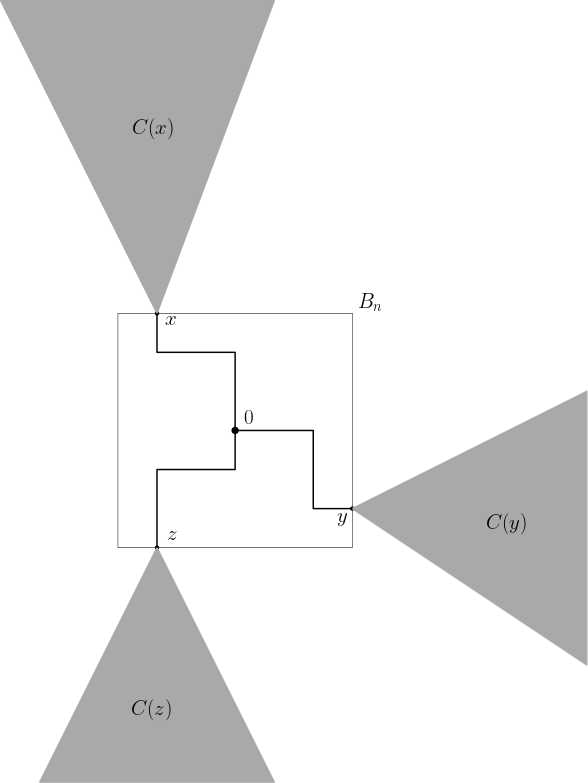
\includegraphics[scale=0.35]{trifconstr.png}
    \caption{Construction (C), the three infinite clusters are represented by gray triangles}
    \label{fig:trif_construct}
\end{figure}

We have by construction

\[ \mathbb{P}_p[\mathscr{T}_0] \geq \frac{1}{2}[p (1 - p)]^{|E_n|}\mathbb{P}_p[N = \infty]. \]

Fix $n \geq 0$ and let $\mathbf{T}$ be the number of trifurcations in $B_n$.
By invariance under translation, we have : $\mathbb{P}_p[\mathscr{T}_x] = \mathbb{P}_p[\mathscr{T}_0]$.

Hence,

\[ \mathbb{E}_p[\mathbf{T}] = |B_n|\times\mathbb{P}_p[\mathscr{T}_0].\]

Now, let us prove that $\mathbf{T} \leq |\partial B_n|$. \ 
We want to construct a family $\{F_0, F_1 ... F_r\}$ by induction where $F_r$ is a forest.
If $F_0 = \{e_1, e_2... e_n\}$ are the edges in $E_n$ open in $\omega$, then

\begin{enumerate}[i)]
\item $\forall 1 \leq i \leq r$, if $e_i$ is in a cycle formed by edges in $F_{i - 1}$, we set $F_i = F_{i - 1} \backslash \{e_i\}$. If not, set $F_i = F_{i - 1}$.

At the end $F_r = \{f_1, ..., f_s\}$ is a forest.
Now we want to construct a family $\{ \Tilde{F}_0, \Tilde{F}_1 ... \Tilde{F}_s \}$ by induction where $\Tilde{F}_s$ is a forest whose leaves belong to $\partial B_n$.

\item $\forall 1 \leq j \leq s$, if $\Tilde{F}_{j - 1}\backslash \{f_j\}$ contains a cluster that does not intersect $\partial B_n$, we set $\Tilde{F}_j = \Tilde{F}_{j - 1} \backslash \{f_j\}$. If not, we set $\Tilde{F}_i = \Tilde{F}_{i - 1}$.

At the end $\Tilde{F}_{s}$ is a forest whose leaves belong to $\partial B_n$.
\end{enumerate}

Notice that trifurcations are preserved from the peeling.

Let $t$ be a trifurcation
\begin{enumerate}[i)]
\item Suppose that there is a cycle in $C(t) \cap B_n$. There are two possibilities. Either a path is joining two branches, and in this case, it is not a trifurcation, because removing edges of $x$ would create less than $3$ clusters, or this cycle is in the same branch, and in this case, there is no problem in removing edges in this cycle because we can bypass and find another path.

\item Suppose that $C(t) \cap B_n$ does not intersect $\partial B_n$. It is impossible since $x_t$, $y_t$ and $z_t$ are in $\partial B_n$.
\end{enumerate}

Therefore trifurcations are conserved and are of the same degree. Trifurcations are vertices of degree $3$ in the forest $\Tilde{F}_s$, which implies that there are less trifurcations than leaves in the forest. Because all of the leaves of $\Tilde{F}_{s}$ belong to $\partial B_n$, we deduce that $\mathbf{T} \leq |\partial B_n|$.

Hence,

\[ \mathbb{P}_p[\mathscr{T}_0] = \frac{\mathbb{E}_p[\mathbf{T}]}{|B_n|} \leq \frac{|\partial B_n|}{|B_n|}\]
which tends to $0$ when $n \longrightarrow \infty$.

Therefore,
\[ \mathbb{P}_p[\mathscr{T}_0] = 0. \]
Since $\mathbb{P}_p[\mathscr{T}_0] \geq \frac{1}{2}[p (1 - p)]^{|E_n|}\mathbb{P}_p[N = \infty]$, we have

\[ \mathbb{P}_p[N = \infty] = 0. \]
Which means that either $N = 0$ or $N = 1$. However $N \not= 0$ almost surely since $\theta(p) > 0$. And that concludes the proof.
\end{proof}

\subsection{Kesten theorem}
The question of the value of $p_c$ remains. We will see that this value is equal to $1/2$ when
$d = 2$ (Theorem \ref{kesten_theorem}). In order to prove this, one step is to prove that for any rectangle $R$ of $\mathbb{Z}^2$, either there exists a left-right path in $R$, or there exists a top-bottom path in $R^h$, but never the two simultaneously. The following proof of the Theorem \ref{kesten_theorem} was taken from an article of Bollobas and Riordan \cite{bollobas}.

\paragraph{Rectangle}
A rectangle $R = [a, b] \times [c,d]$ is the induced subgraph of $\mathbb{Z}^2$ where $a < b$, $c < d$ integers. This subgraph includes all vertices and edges in the interior and boundary of $R$.

The horizontal dual $R^h = [a + 1/2, b - 1/2] \times [c - 1/2,d + 1/2]$ is the subgraph of $(Z^2)^*$ including all vertices and edges in the interior and boudary of $R^h$.

\begin{lemma}
\label{lr_tb_lemma}
Let $R$ be a rectangle.

We call 
\[\mathscr{H}(R) = \{R \text{ contains a left-right path}\}.\]
and
\[\mathscr{V^*}(R^h) = \{R^h \text{ contains a top-bottom path}\}.\] 

For every configuration $\omega \in \{ 0, 1 \}^\mathbb{N}$, either $\mathscr{H}(R)$ or $\mathscr{V^*}(R^h)$ is true.
\end{lemma}
\begin{proof}

Let us define the following variables

\[ \Tilde{L} = (0, 2) + 4 \mathbb{Z}^2. \]
\[ \Tilde{L^*} = (2, 0) + 4 \mathbb{Z}^2. \]
\[ \Tilde{R} = \{ (4i, 4j + 2) : 0 \leq i \leq k \text{ and } 0 \leq j \leq l - 1 \}. \]
\[ \Tilde{R^h} = \{ (4i + 2, 4j) : 0 \leq i \leq k - 1 \text{ and } 0 \leq j \leq l \}. \]

\[ R_{m} = \{ (2i + 1, 2j + 1 : 0 \leq i \leq 2k - 1 \text{ and } 0 \leq j \leq 2l - 1\}. \]

The entire construction is represented in Figure \ref{fig:lr_thm}.
Let $G$ be the subgraph formed by $\Tilde{R}$ and $G^h$ be the subgraph formed by $\Tilde{R}^h$.

We construct $M$ the middle graph between $G$ and $G^h$ .

$M$ is defined as the subgraph with vertices $R_{m}$ and such that one vertex is connected to one another if and only if it does not cross a vertex of $G$ or $G^h$. We orient edges such that $G$ is on the right and $G^h$ is on the left.

We can observe that any vertex of $M$ is of degree $2$ except the corners $x, y, z, w$ that are of degree $1$ (top-left, bottom-left, bottom-right, top-right resp.). 

If we choose this orientation, we obtain that $x$ and $z$ are entry points and $y$ and $w$ exit points.

Thus if we look the connected subgraph of $x$ in $M$, we can see that it is a path $P$. $P$ endpoint being either $y$ or $w$. 

\begin{itemize}
    \item If $P$ endpoint is $w$, then all of the edges of $G$ to the right of $P$ form a connected subgraph, which means that there exists a left-right path in $G$.
    \item If $P$ endpoint is $y$, then all of the edges of $G^h$ to the right of $P$ form a connected subgraph, which means that there exists a top-bottom path in $G^h$.
\end{itemize}

That means that at least one of the events $\mathscr{H}(\Tilde{R})$ or $\mathscr{V^*}(\Tilde{R^h})$ holds.

Now let us prove that only one of them holds for every configuration. Since $P$ is a simple path, we can construct a simple closed curve $\overline{P}$ by rejoining $x$ and $w$ in the top. All top edges of $G$ being contained in the interior region delimited by $\overline{P}$, if a bottom-right path would exist, that would mean it would cross this region, and therefore $\overline{P}$ which is a subgraph of $M$, which contradicts the definition of $M$. We have to notice that although if uses the Jordan's theorem, it only needs to use the easy part.

Therefore one and only one of the events $\mathscr{H}(\Tilde{R})$ and $\mathscr{V^*}(\Tilde{R^h})$ holds. And that concludes the proof.
\begin{figure}
    \centering
    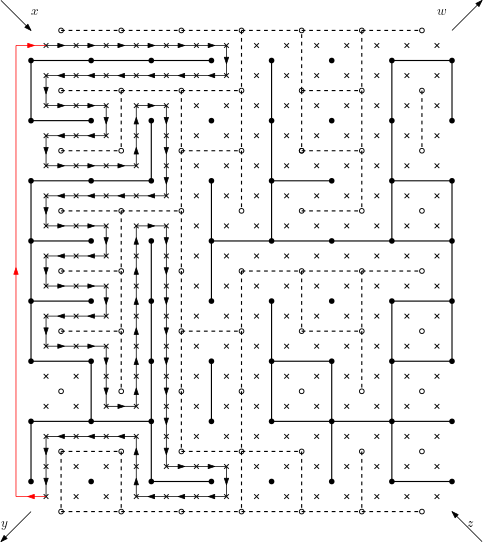
\includegraphics{graph_kesten}
    \caption{Graph $G$ (black vertices and solid edges), $G^h$ (white vertices and dashed edges) and $M$ (crossed vertices, and not all edges shown), $P$ is the black path with arrows and by joining $x$ and $y$ in the red path, we obtain the closed path $\overline{P}$}
    \label{fig:lr_thm}
\end{figure}
\end{proof}
\begin{lemma}
\label{Hn1half_lemma}
Let $\mathscr{H}_n$ be the event that there exists a self-avoiding left-right path going through $R_n = [0, n] \times [0, n - 1]$.

Let $\mathscr{V}_n$ be the event that there exists a self-avoiding top-bottom path going through $R'_n = [0, n - 1] \times [0, n]$.

We have

\[ \forall n \geq 1, \mathbb{P}_p[\mathscr{H}_n] + \mathbb{P}_{p}[\mathscr{V}_n] = 1. \]

For $p = \frac{1}{2}$, we have

\[ \forall n \geq 1, \mathbb{P}_{1/2}[\mathscr{H}_n] = \mathbb{P}_{1/2}[\mathscr{V}_n] = \frac{1}{2}. \]
\end{lemma}
\begin{proof}
Lemma \ref{lr_tb_lemma} gives us the first formula
\[ \forall n \geq 1, \mathbb{P}_p[\mathscr{H}_n] + \mathbb{P}_{p}[\mathscr{V}_n] = 1. \]

If we set $p = 1 / 2$, the two probabilities are equal and we obtain the second equation
\[ \mathbb{P}_{1/2}[\mathscr{H}_n] = \mathbb{P}_{1/2}[\mathscr{V}_n] = \frac{1}{2}. \]
And that concludes the proof.
\end{proof}

Since the two lemmas have been proven, we can attack the Kesten's theorem.
\begin{theorem}[Kesten's theorem]
\label{kesten_theorem}
  For Bernoulli bond percolation on $\mathbb{Z}^2$, $p_c=1/2$. Moreover there is no infinite cluster at $p_c$.
\end{theorem}
\begin{proof}
Set $p = \frac{1}{2}$.

Using the lemma \ref{Hn1half_lemma}, we have
\[ \mathbb{P}_p[\mathscr{H}_n] = \frac{1}{2}. \]

Hence,
\[ \lim_{n \rightarrow \infty}{\mathbb{P}_p[\mathscr{H}_n]} = \frac{1}{2}.\]

Which is distinct from $1$, which means that $\theta(\frac{1}{2}) = 0$ and $p_c \geq \frac{1}{2}$ and is distinct from $0$, which means that $p_c \leq \frac{1}{2}$.

Therefore $p_c = \frac{1}{2}$.
\end{proof}

\section{Simulation}
I have made a program in Python that simulates the Bernoulli bond percolation on a $\mathbb{Z}^2$ lattice in a $N$-box for a given $p \in [0,1]$.

This program uses the library \lstinline[language=Python]{pygame} to display graphics. It uses breadth first search algorithm to find open clusters, and colorizes them with the biggest one in red.

\subsection{Model used}
We represent the lattice $\mathbb{Z}^2$ in a $N \times N$ rectangle by an array of integers $N \times N$ where each element is a list of $5$ integers. The fourth first integers represent the state of the edges in this order: right, up, left, down. If the value is $0$, that means the edge is closed and if it is equal to $1$, that means the edge is open. Thus, any edge not on the bounds is represented two times by its two endpoints. The fifth value is used to represent at which cluster the vertex belongs.

\subsection{Breadth-first search algorithm}
Breadth-first search algorithm is an efficient method to find open clusters. This was the method chosen rather than depth-first search algorithm, it is more suitable because we have to explore all connected vertices and we don't have too much recursion.

\subsubsection{General case}
Breadth-first search algorithm is an algorithm that explores a given graph $G = (V,E)$. A list \lstinline[language=Python]{lst} of all visited vertices is created. The goal is to visit every vertex only one time in order to avoid cycles. In other words, we find a tree subgraph $T$ of $G$. It explores nodes of $T$ at the same depth prior to moving on to the nodes at the next depth level.

The function \lstinline[language=Python]{bfs} takes as an input \{\lstinline[language=Python]{G, v, queue, lst}\} such that \lstinline[language=Python]{G} is the graph explored, \lstinline[language=Python]{v} is a given vertex, \lstinline[language=Python]{queue} the LIFO queue of vertices to explore and  \lstinline[language=Python]{lst} the list of visited vertices. It first marks all of the neighbours of  \lstinline[language=Python]{v}, and add them to  \lstinline[language=Python]{queue} and then explores all of the neighbours of the first element of \lstinline[language=Python]{queue}, and so on. For instance, this algorithm is applied on a graph in Figure \ref{tab:bfs_graph}.

\begin{figure}
\centering
\caption{Application of BFS algorithm for a graph}
\begin{tabular}{cc}
\label{tab:bfs_graph}
    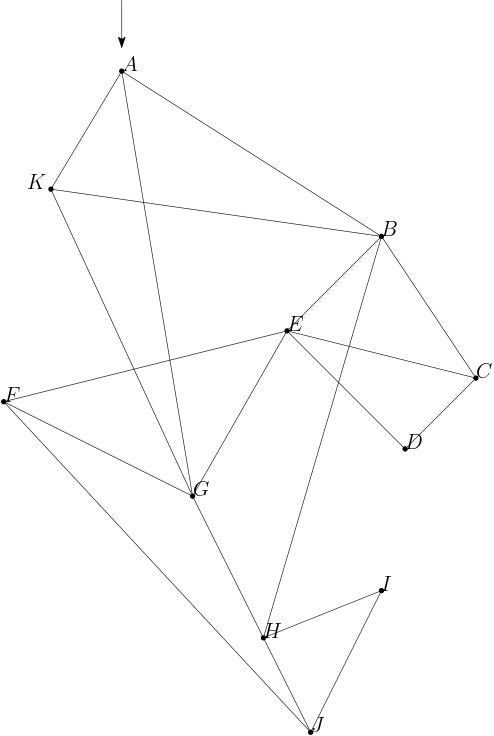
\includegraphics[scale=0.5]{graph} & 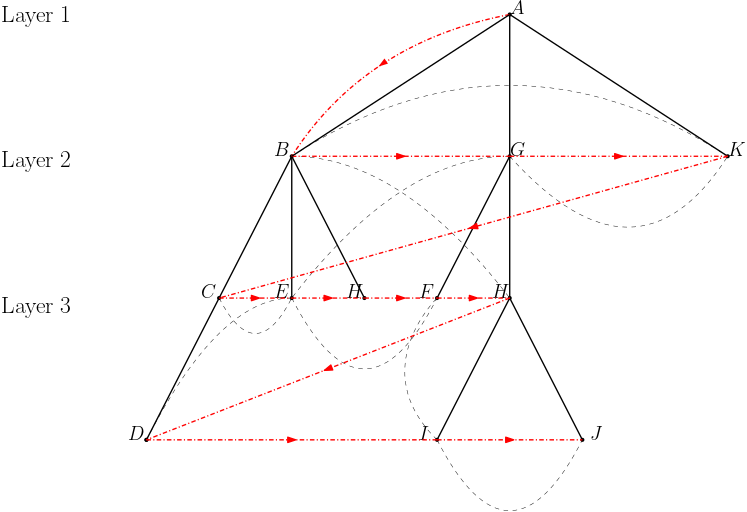
\includegraphics[scale=0.35]{treegraph} \\
Examples of a graph $G$ of $11$ vertices & Graph $G$ where $T$ is in solid black edges \\
& edges not used are in dashed black edges \\
& the path used by the algorithm is in red
\end{tabular}
\end{figure}

\subsubsection{Application for the search of open clusters}
As we mentioned earlier, we will use this algorithm in order to find open clusters of $\omega \in \{0,1\}^\mathbb{E}$, which is the same as finding connected components of $K(\omega)$. In order to find connected components of $K(\omega)$, we have to modify our algorithm. For each connected component is associated a unique id strictly greater than $0$. The id $0$ is reserved for non-explored vertices.

Thus there are two functions \lstinline[language=Python]{bfs_subiterative} and \lstinline[language=Python]{bfs_iterative}. \lstinline[language=Python]{bfs_iterative} explores the vertices of the lattice $\mathbb{Z}^2$ one by one, left to right, top to bottom. It uses a counter \lstinline[language=Python]{count} for the ids of open clusters. Each time a vertex \lstinline[language=Python]{v = (x,y)} is encountered, the counter increases by $1$ if and only if the associated open cluster id of \lstinline[language=Python]{v} in \lstinline[language=Python]{state} is equal to $0$. \lstinline[language=Python]{bfs_subiterative} acts like \lstinline[language=Python]{bfs} for a vertex \lstinline[language=Python]{v = (x,y)} with a given cluster id  \lstinline[language=Python]{mark = count} with no list \lstinline[language=Python]{lst} because we use the fifth value of each element of \lstinline[language=Python]{state}, we know that it was not visited if and only if this value is equal to $0$. When we visit this vertex, we replace the fifth value from $0$ to \lstinline[language=Python]{mark}. Furthermore, two variables \lstinline[language=Python]{maxid} and \lstinline[language=Python]{maxcount} are created in order to represent the biggest cluster with \lstinline[language=Python]{maxid} the id of the biggest cluster and \lstinline[language=Python]{maxcount} the number of vertices of this cluster. The function \lstinline[language=Python]{bfs_iterative} returns this variable \lstinline[language=Python]{maxid}.

Here is the code of the BFS algorithm:
\lstinputlisting[language=Python]{bfs_algorithm.py}

\subsection{Code of the program}
The entire program consists of seven functions. \lstinline[language=Python]{bfs_iterative} and \lstinline[language=Python]{bfs_subiterative} finds the open clusters. The function \lstinline[language=Python]{neighbours} returns a list of neighbours for a given vertex \lstinline[language=Python]{v = (x,y)}. The function \lstinline[language=Python]{delete} opens a given edge and \lstinline[language=Python]{show} draws the lattice $\mathbb{Z}^2$ with open edges colored with random colors for each open cluster. 

The function \lstinline[language=Python]{initialize} creates a blank lattice $\mathbb{Z}^2$ with all edges closed and all ids of open clusters equal to $0$. The function \lstinline[language=Python]{percolate} open each edge for a given probability $p \in [0,1]$.

Here is the entire code of the program:
\lstinputlisting[language=Python]{percolationWindow.py}

\subsection{Results}
Here are some given outputs in Figure \ref{tab:simulation} for the bond percolation on $\mathbb{Z}^2$ for $p = 0.2$, $p = 0.4$, $p = 0.5$, $p = 0.6$, $p = 0.8$.

We can clearly observe that as $p$ tends to $1$, the biggest is the cluster in red, and that the more $p$ tends to $0$, the diameter of the open clusters decays exponentially. Finally we can see that $p_c = 1/2$ is the critical value.
\begin{figure}
\centering
\caption{Outputs of the program for different parameters}
\begin{tabular}{cc}
\label{tab:simulation}
  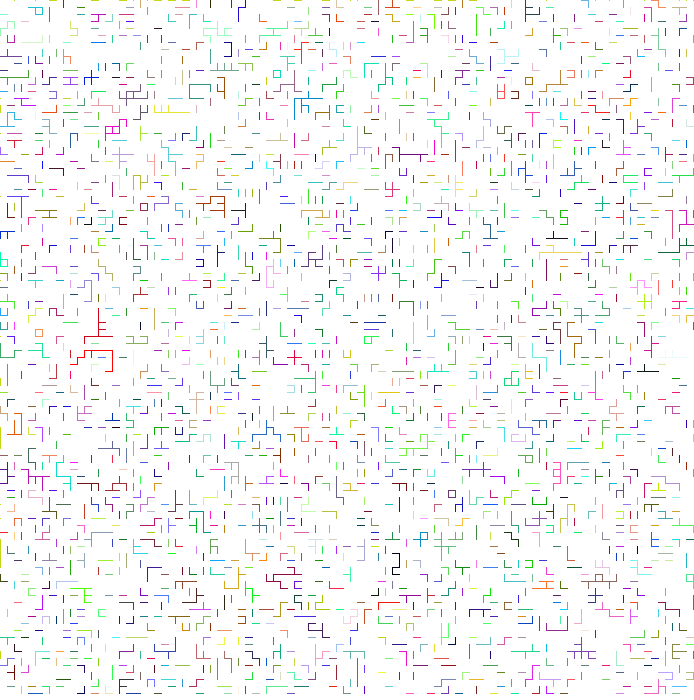
\includegraphics[width=55mm]{p20} &   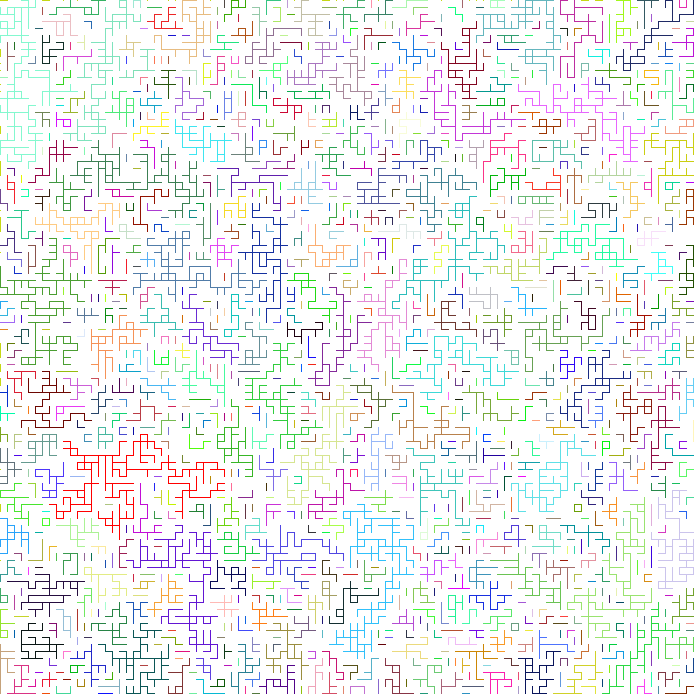
\includegraphics[width=55mm]{p40} \\
$p = 0.2$, Size = $100 \times 100$ & $p = 0.4$, Size = $100 \times 100$  \\[6pt]
 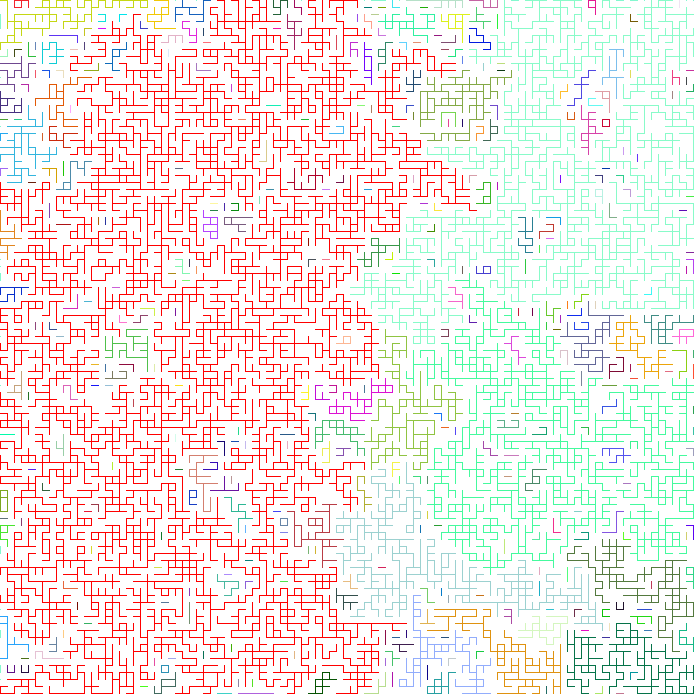
\includegraphics[width=55mm]{p50} &   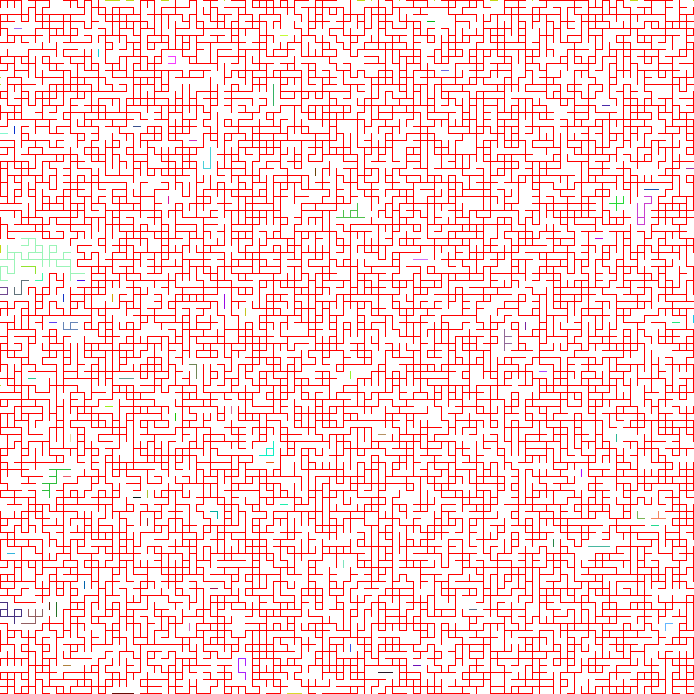
\includegraphics[width=55mm]{p60} \\
$p = 0.5$, $\text{Size} = 100 \times 100$ & $p = 0.6$, Size = $100 \times 100$  \\[6pt]
\multicolumn{2}{c}{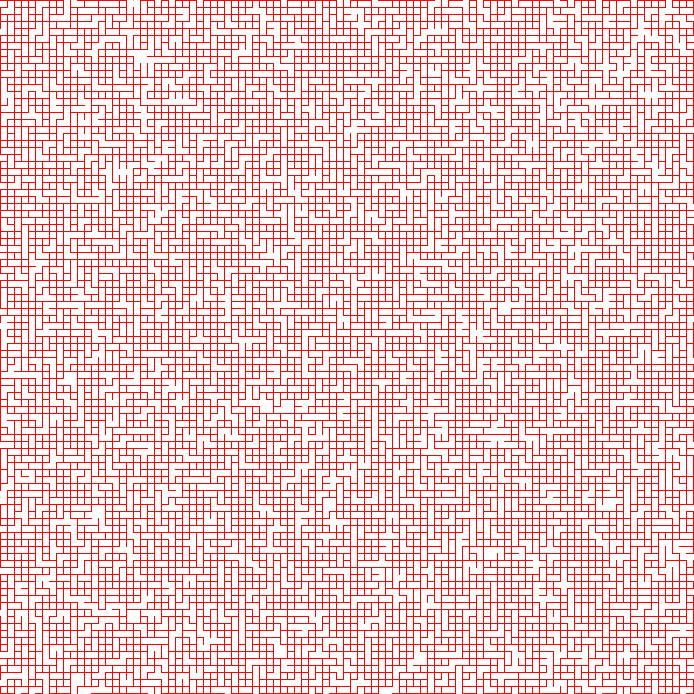
\includegraphics[width=55mm]{p80} }\\
\multicolumn{2}{c}{$p = 0.8$, Size = $100 \times 100$}
\end{tabular}
\end{figure}

\medskip

\newpage
\printbibliography[heading=bibintoc,title={References}]


\end{document}